\section{Kristalloscillatorer}
\textbf{HAREC a.\ref{HAREC.a.3.6.4}\label{myHAREC.a.3.6.4}}
\index{kristalloscillator}
\index{oscillator!kristalloscillator}

\subsection{Kvartskristaller i oscillatorkopplingar}
\index{XO}
\index{oscillator!XO}
\index{VFO}
\index{oscillator!VFO}

En LC-oscillators frekvensstabilitet begränsas av de ingående
komponenternas egenskaper.
När mycket bättre stabilitet än så krävs, speciellt inom stora
temperaturområden, så är kvartskristallen en svängningskrets med bättre data.
Kvartskristallens höga Q-värde ger också en renare signal.

\begin{wrapfigure}{R}{0.5\textwidth}
  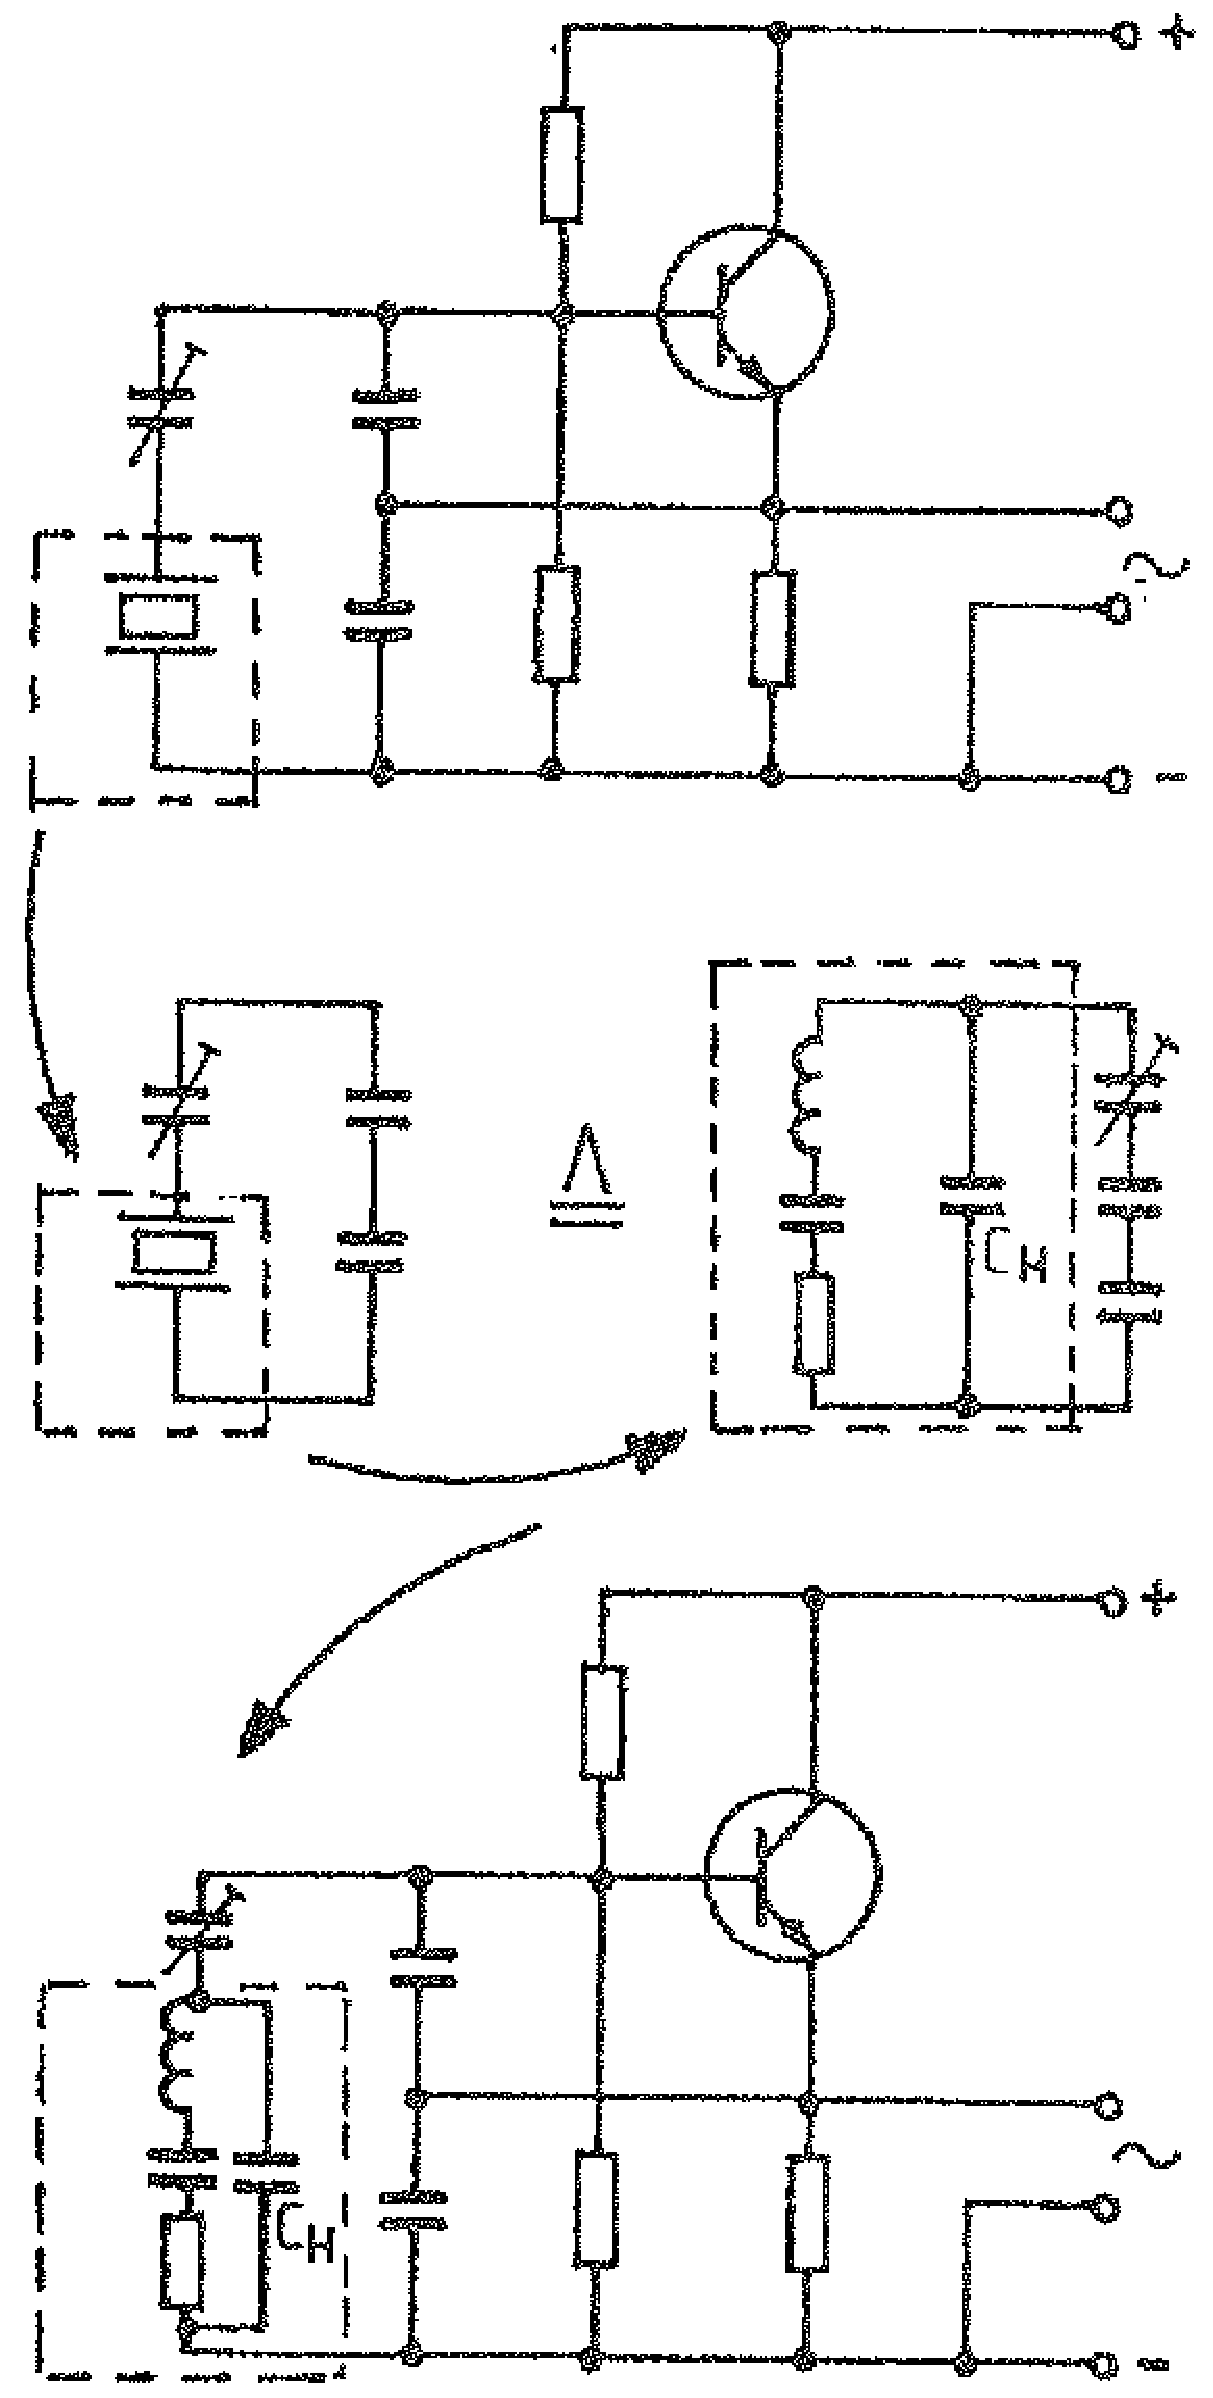
\includegraphics[width=0.5\textwidth]{images/cropped_pdfs/bild_2_3-75.pdf}
  \caption{Colpittsoscillator med kristall i parallellresonansfallet}
  \label{fig:BildII3-75}
\end{wrapfigure}

I en \emph{kristalloscillator} (eng. \emph{Crystal Oscillator (XO)}) är en
kvartskristall det frekvensbestämmande elementet i stället för en LC-krets.
I övrigt kan samma kopplingsprinciper som för en LC-VFO användas.

Kristallen kan utföras så att den svänger antingen som en serie- eller
parallellresonanskrets.
Märk, att en kristall svänger på något olika frekvens beroende på om den fås
att fungera som serie- eller parallellkrets.
Den högre frekvensen är den som vanligen används.

Bild \ref{fig:BildII3-75} visar en Colpittoscillator med en kristall i
parallellresonansfallet.
I parallellresonansalternativet kopplas kristallen parallellt över
oscillatorns återkopplingsled.
Den minsta dämpningen av den återkopplade signalen fås när signalens frekvens
är lika kristallens resonansfrekvens.
Kristallens reaktans är då som högst.

Parallellt över kristallens inre induktans ligger dess inre
seriekopplade kapacitanser \(C\) och \(C_H\).
Yttre kapacitanser (en trimbar och två fasta kondensatorer i serie) är kopplade
parallellt över den inre anslutningskapacitansen \(C_H\).

Om den trimbara kapacitansen ändras, så påverkas kristallens resonansfrekvens.
Man säger då att man ''drar'' kristallen inom ett litet frekvensområde.
Kristallens och oscillatorns egenskaper avgör hur stort området kan vara.
Om kristaller dras för mycket, så kan resonansfrekvensen bli ostabil.
Den relativa frekvensändringen uppgår till högst \(10^{-4} = 0,01\%\).
Formel:

\[
\text{relativ frekvensändring} =
\frac{\text{absolut ändring}}{\text{resonansfrekvens}}
\]

\subsection{Övertonskristaller}
\index{övertonskristall}
\index{kristal!övertonskristall}

\begin{wrapfigure}{R}{0.5\textwidth}
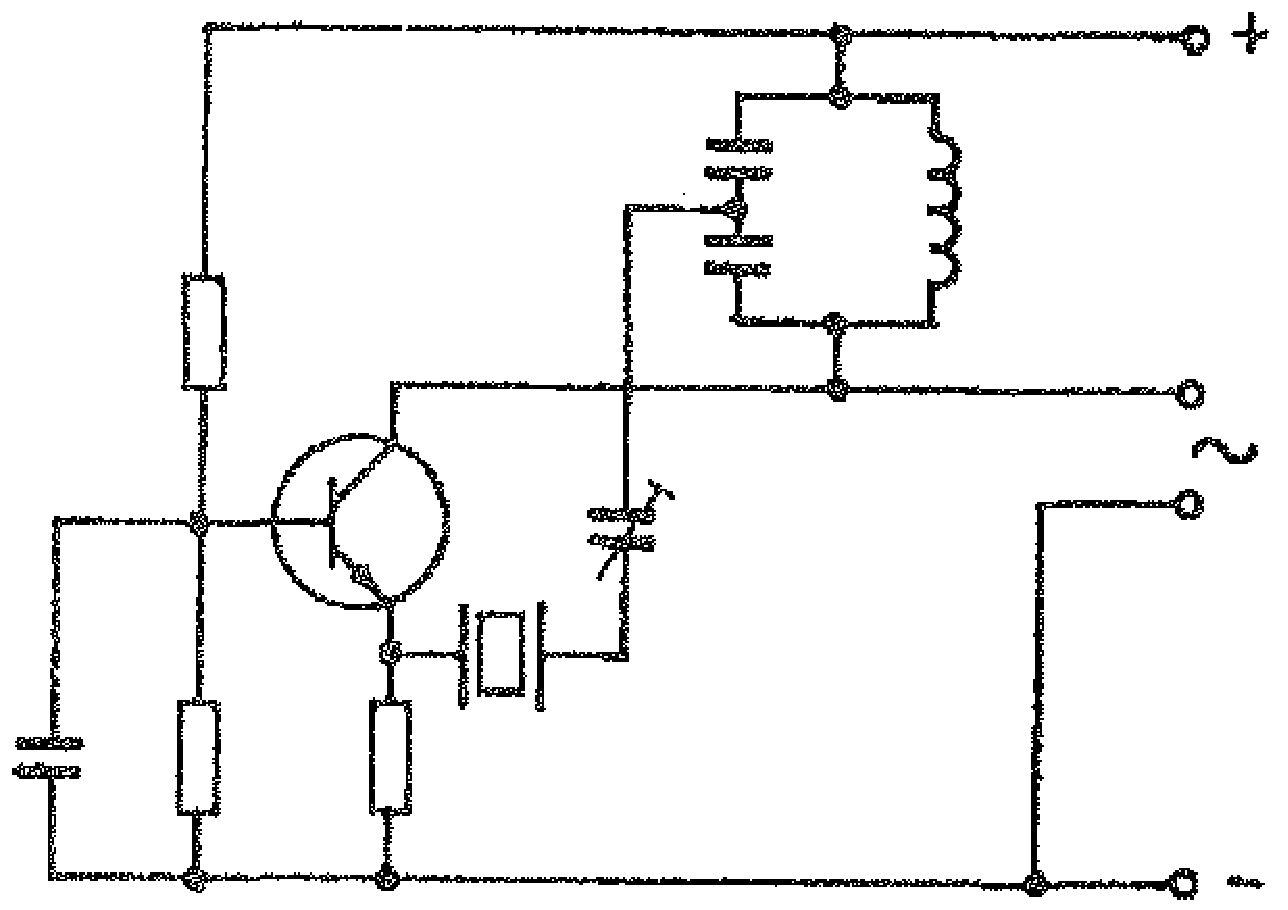
\includegraphics[width=0.5\textwidth]{images/cropped_pdfs/bild_2_3-76.pdf}
\caption{Colpittsoscillator med kristall i serieresonansfallet}
\label{fig:BildII3-76}
\end{wrapfigure}

Bild \ref{fig:BildII3-76} visar en Colpittsoscillator med kristall i
serieresonansfallet.
I serieresonansalternativet kopplas kristallen in i serie med
oscillatorns återkopplingsled.
Den minsta dämpningen av den återkopplade utgångssignalen fås, när signalens
frekvens är lika som kristallens resonanfrekvens.
Kristallens reaktans är då som lägst.
Så kallade övertonskristaller används för oscillatorfrekvenser över ca 20~MHz.

Övertonskristallernas dimensioner är lika grundtonskristallernas, men
snittas ut annorlunda och slipas för att svänga på önskad udda överton.
En övertonskristall har övertonens frekvens instämplad i höljet och kristallen
förutsätts arbeta i oscillatorkopplingar som seriekrets.
Genom att låta kristaller svänga på sin överton undviker man en svår
tillverkningsprocedur, nämligen att slipa mycket tunna kristallskivor.

En övertonsoscillator måste alltid innehålla en svängningskrets som är
avstämd till den överton som anges på kristallen.

\textbf{Modellförsök:}
En instrumentsträng sätts i svängning på sin grundton genom en knäppning mitt
på strängen.
En knäppning på en punkt bort från mitten får strängen att svänga på en överton
i stället.

\subsection{Superheterodyn-VFO}
\index{superheterodyn!VFO}
\index{oscillator!syperheterodyn-VFO}

\begin{figure}
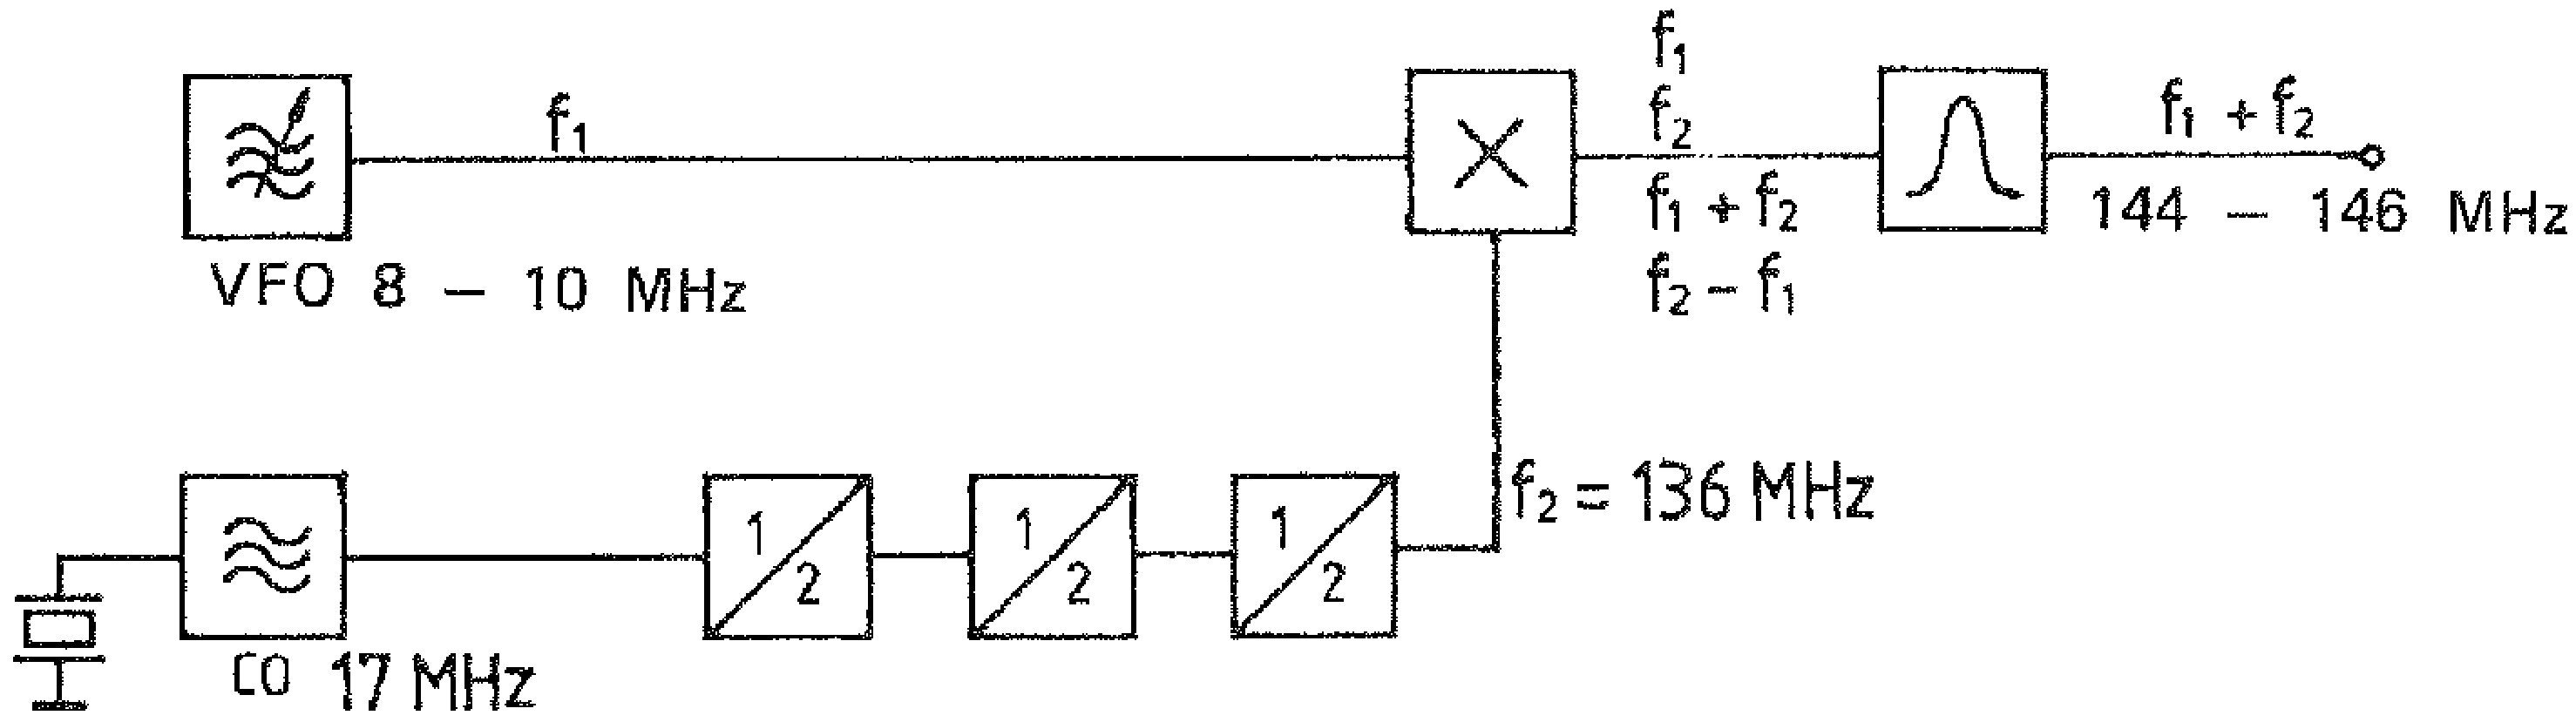
\includegraphics[width=\textwidth]{images/cropped_pdfs/bild_2_3-77.pdf}
\caption{Superheterodyn-VFO}
\label{fig:BildII3-77}
\end{figure}

Bild \ref{fig:BildII3-77} visar en Superheterodyn-VFO.
En enkel LC-VFO är inte tillräckligt frekvensstabil i ett högt frekvensläge,
till exempel 144--146~MHz.
Man kan då använda en speciell koppling, som är en kombination av LC-VFO och
XO, kallad super-VFO.

I en super-VFO blandas en låg, variabel frekvens från en VFO med en hög
frekvens från en XO.
Ordet super kommer från superheterodyne = överlagring, blandning.
En VFO arbetar stabilare på låg frekvens medan en XO fortfarande arbetar
stabilt även på högre frekvenser, dock inte så högt som vi behöver här.
I vårt exempel arbetar därför VFO i området 8--10~MHz och XO på 17~MHz.
VFO-signalen blandas med en fast signalfrekvens, som är XO-signalen 17~MHz
multiplicerat med 8, det vill säga 136~MHz.

Ett bandpassfilter filtrerar fram den önskade blandningsprodukten, som
ligger i frekvensområdet 144--146~MHz.
Resultatet blir en hög frekvens, som är både variabel och stabil.

\textbf{Fördelar:}
Frekvensstabiliteten hos en super-VFO är mycket bättre än hos en enkel VFO,
som arbetar direkt i VHF-området.
En super-VFO är dessutom mycket brusfattigare än en PLL-VFO, vilken
beskrivs här nedan.

\textbf{Nackdelar:}
Vid frekvensblandning uppstår oönskade blandningsprodukter, vilka visserligen
dämpas av bandpassfilter, men som det är omöjligt att undertryckta helt.
Bland annat alstras en svag spegelfrekvens, som vandrar från 128 till 126~MHz,
samtidigt som den önskade blandningsprodukten vandrar från 144 till 146~MHz.
Risken för att spegelfrekvensen förstärks och sänds ut måste elimineras,
vilket kan göras med effektiva bandpassfilter.
Se vidare i avsnitt \ref{blandare} om frekvensblandning.

\subsection{Oscillatorer med faslåsning (PLL)}
\textbf{HAREC
  a.\ref{HAREC.a.3.7}\label{myHAREC.a.3.7}
}
\index{PLL}
\index{Phase Locked Loop (PLL)}

En kristalloscillator (XO) arbetar med god frekvensstabilitet.
Frekvensen som är fast bestäms av styrkristallen.

En LC-oscillator arbetar däremot inom ett frekvensområde (VFO), som
bestäms av en LC-krets.
Dennas frekvens är emellertid mindre stabil än den med styrkristall.

I en \emph{fas-låst loop} (eng. \emph{Phase Locked Loop (PLL)}) kan god
frekvenstabilitet och stort frekvensområde förenas.
En PLL är en sluten krets för elektrisk styrning av en oscillator, så att dess
frekvens är både stabil och variabel.

\subsubsection{Spänningsstyrd oscillator (VCO)}
\textbf{HAREC a.\ref{HAREC.a.3.6.5}\label{myHAREC.a.3.6.5}}
\index{spänningsstyrd oscillator}
\index{oscillator!spänningsstyrd}
\index{VCO}
\index{oscillator!VCO}
\index{VFO}
\index{oscillator!VFO}

I bild \ref{fig:BildII3-78} jämförs en VFO och en VCO.
En VFO, vars frekvens kan styras med en likspänning, kallas
\emph{spänningstyrd oscillator} (eng. \emph{Voltage Controlied Oscillator
  (VCO)}).
I svängningskretsen i en VCO fyller en kapacitansdiod (varicap, variable
capacitor) samma uppgift som den mekaniskt variabla kondensatorn i en VFO.

\begin{wrapfigure}[43]{R}{0.5\textwidth}
  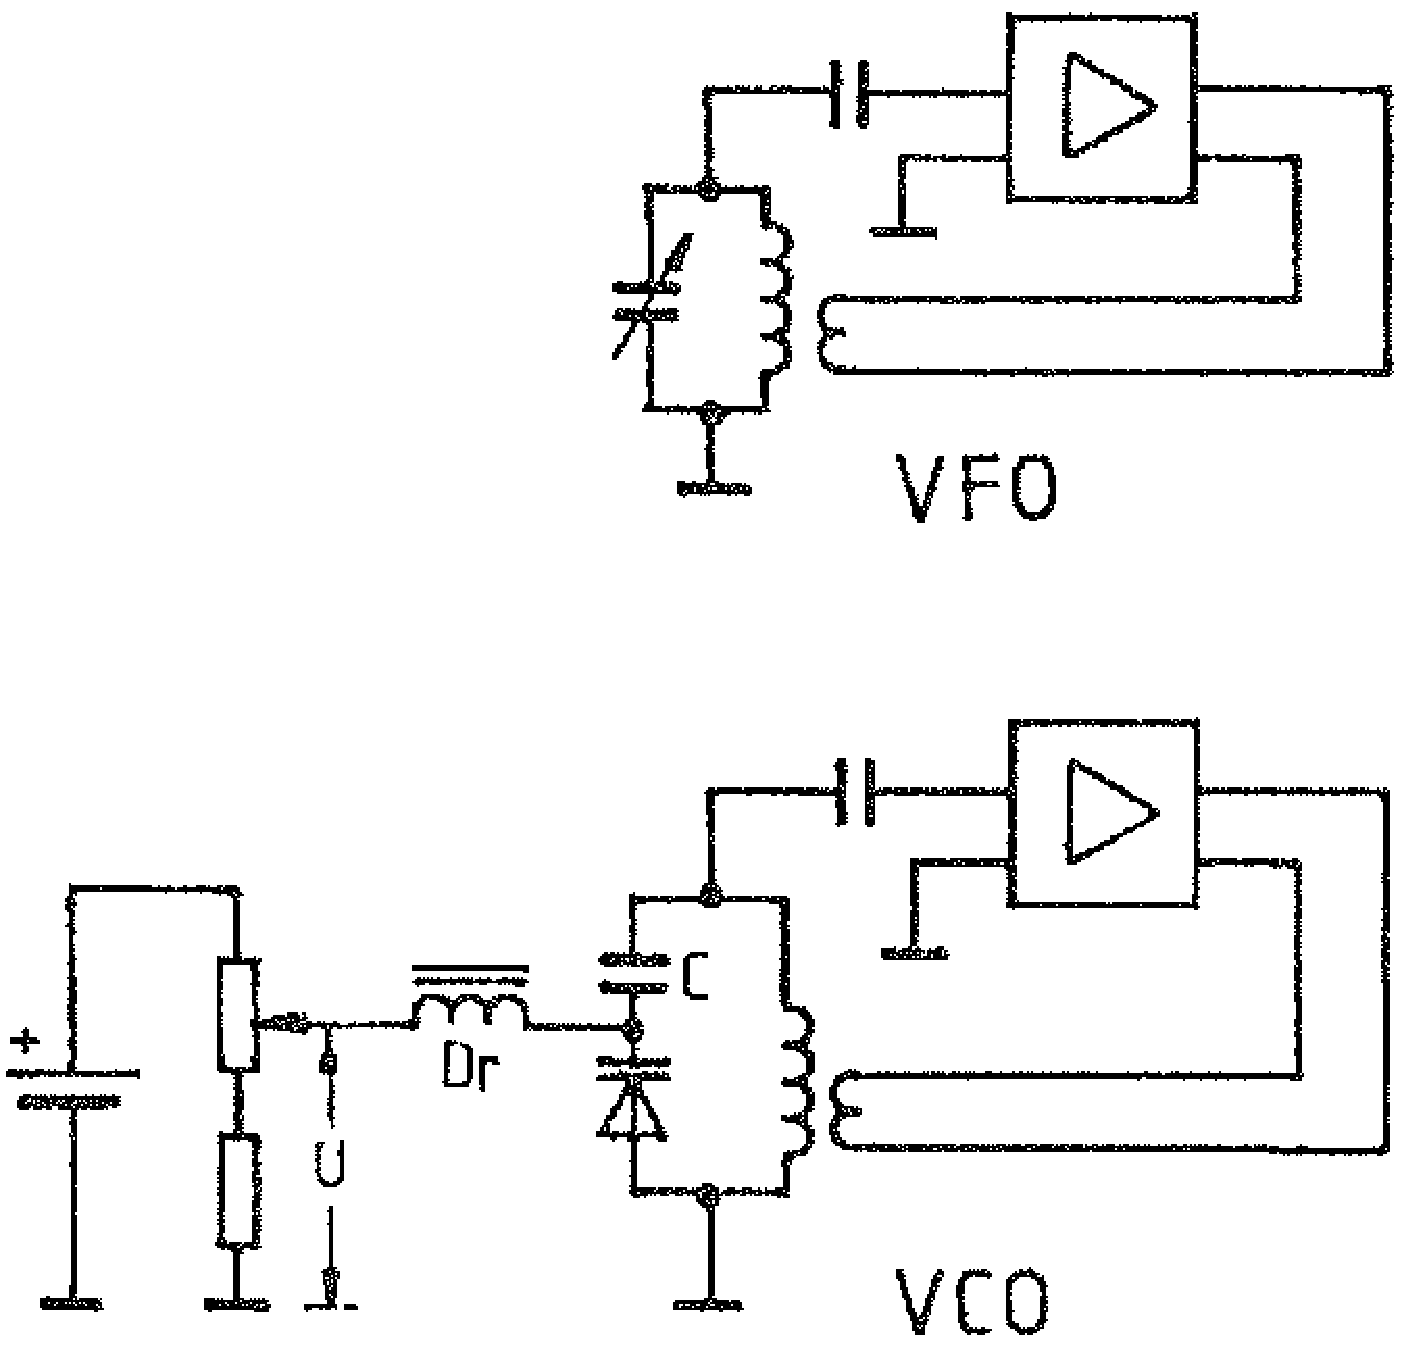
\includegraphics[width=0.5\textwidth]{images/cropped_pdfs/bild_2_3-78.pdf}
  \caption{VFO och VCO jämförs}
  \label{fig:BildII3-78}

  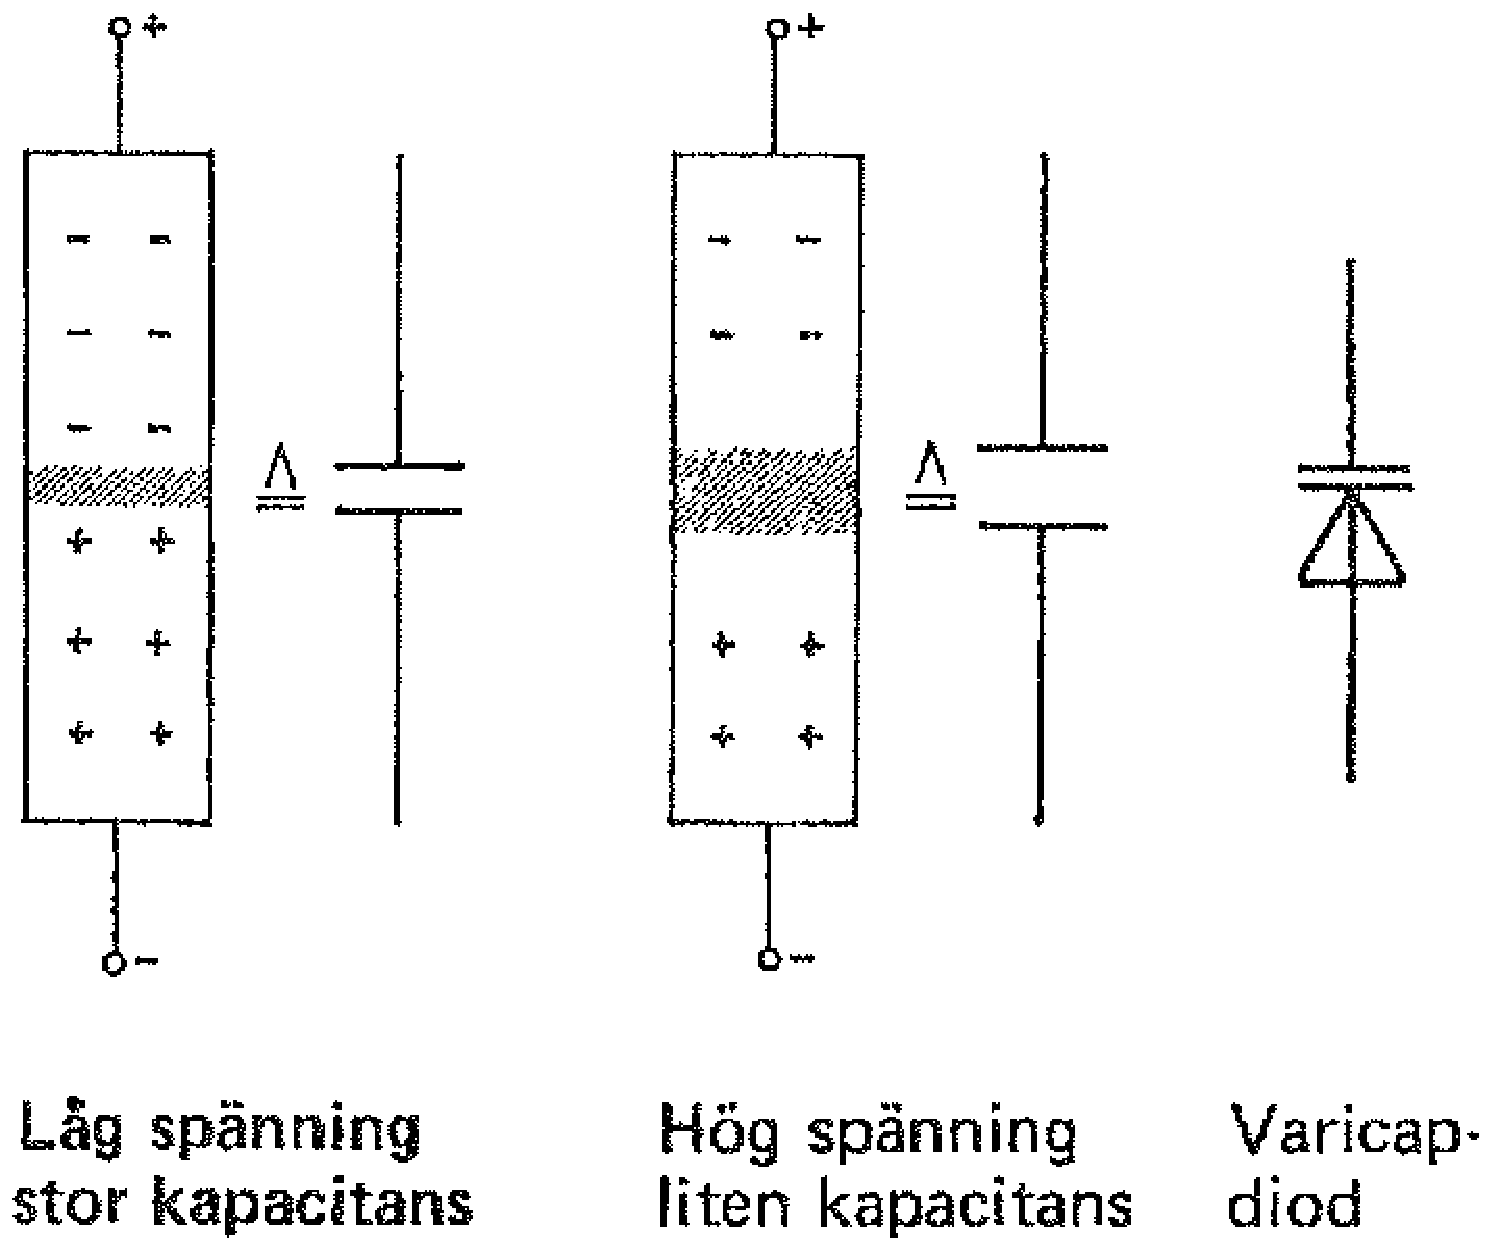
\includegraphics[width=0.5\textwidth]{images/cropped_pdfs/bild_2_3-79.pdf}
  \caption{Kapacitansdiod -- Varicap}
  \label{fig:BildII3-79}

  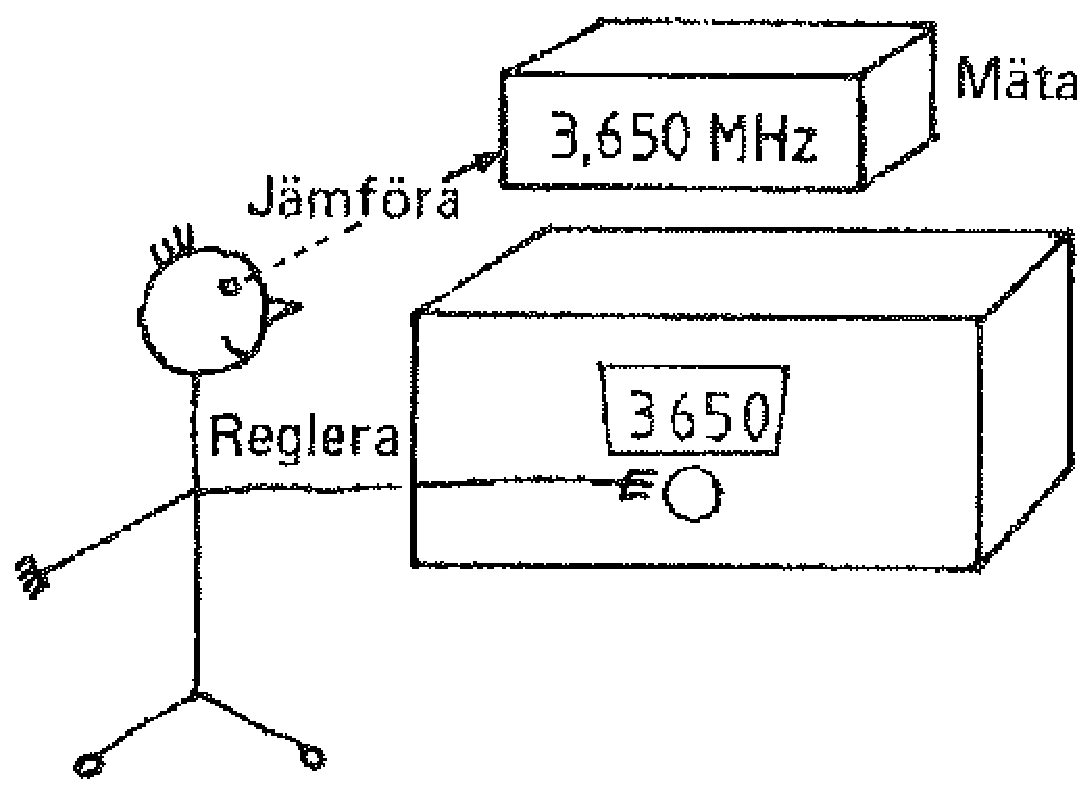
\includegraphics[width=0.5\textwidth]{images/cropped_pdfs/bild_2_3-80a.pdf}
  \caption{Analogi Människa-PLL}
  \label{fig:BildII3-80a}
\end{wrapfigure}

Bild \ref{fig:BildII3-79} visar en kapacitansdiod -- varicap.
När en motriktad spänning läggs på dioden, så bildas ett spärrskikt i dioden,
så att zonerna med fria laddningsbärare isoleras från varandra likt
kondensatorplattor.
Spärrskiktets tjocklek (ca 1/1000~mm) beror av spänningen över dioden.
Vid hög spänning är spärrskiktet tjockt, vilket motsvarar
''stort plattavstånd'' och liten kapacitans.
Vid låg spänning är skiktet tunt, vilket motsvarar ''litet plattavstånd'' och
stor kapacitans.

Med en kapacitansdiod i svängningskretsen, i stället för en mekaniskt
variabel kondensator, så behövs ytterligare två komponenter.
Drosseln \(D_r\) hindrar högfrekvenssignalen att överlagras på styrkretsens
likspänning.
Då skulle bland annat svängningskretsens godhetstal försämras (förlorad HF-energi
innebär dämpning).
Omvänt hindrar kondensatorn \(C\) att dioden och spärrspänningen kortsluts genom
induktorn.
Oscillatorfrekvensen ställs in med den variabla likspänningen \(U\).
Av en VFO har det blivit en VCO.

\subsubsection{Oscillator med PLL-styrning}
\textbf{HAREC a.\ref{HAREC.a.3.7.1}\label{myHAREC.a.3.7.1}}

Bild \ref{fig:BildII3-80a} visar en manuell frekvensstyrning.
Människan jämför och reglerar förlopp utifrån givna fakta.
Det kan liknas med PLL-kretsens sätt att jämföra det inbördes fasläget mellan
signalen från en VCO (är-värdet) och signalen från en XO (bör-värdet).

Som resultat av jämförelsen justeras styrspänningen så att är- och
bör-frekvenserna hålls lika.
En sådan reglerkrets består av digitala komponenter.

\begin{figure}
  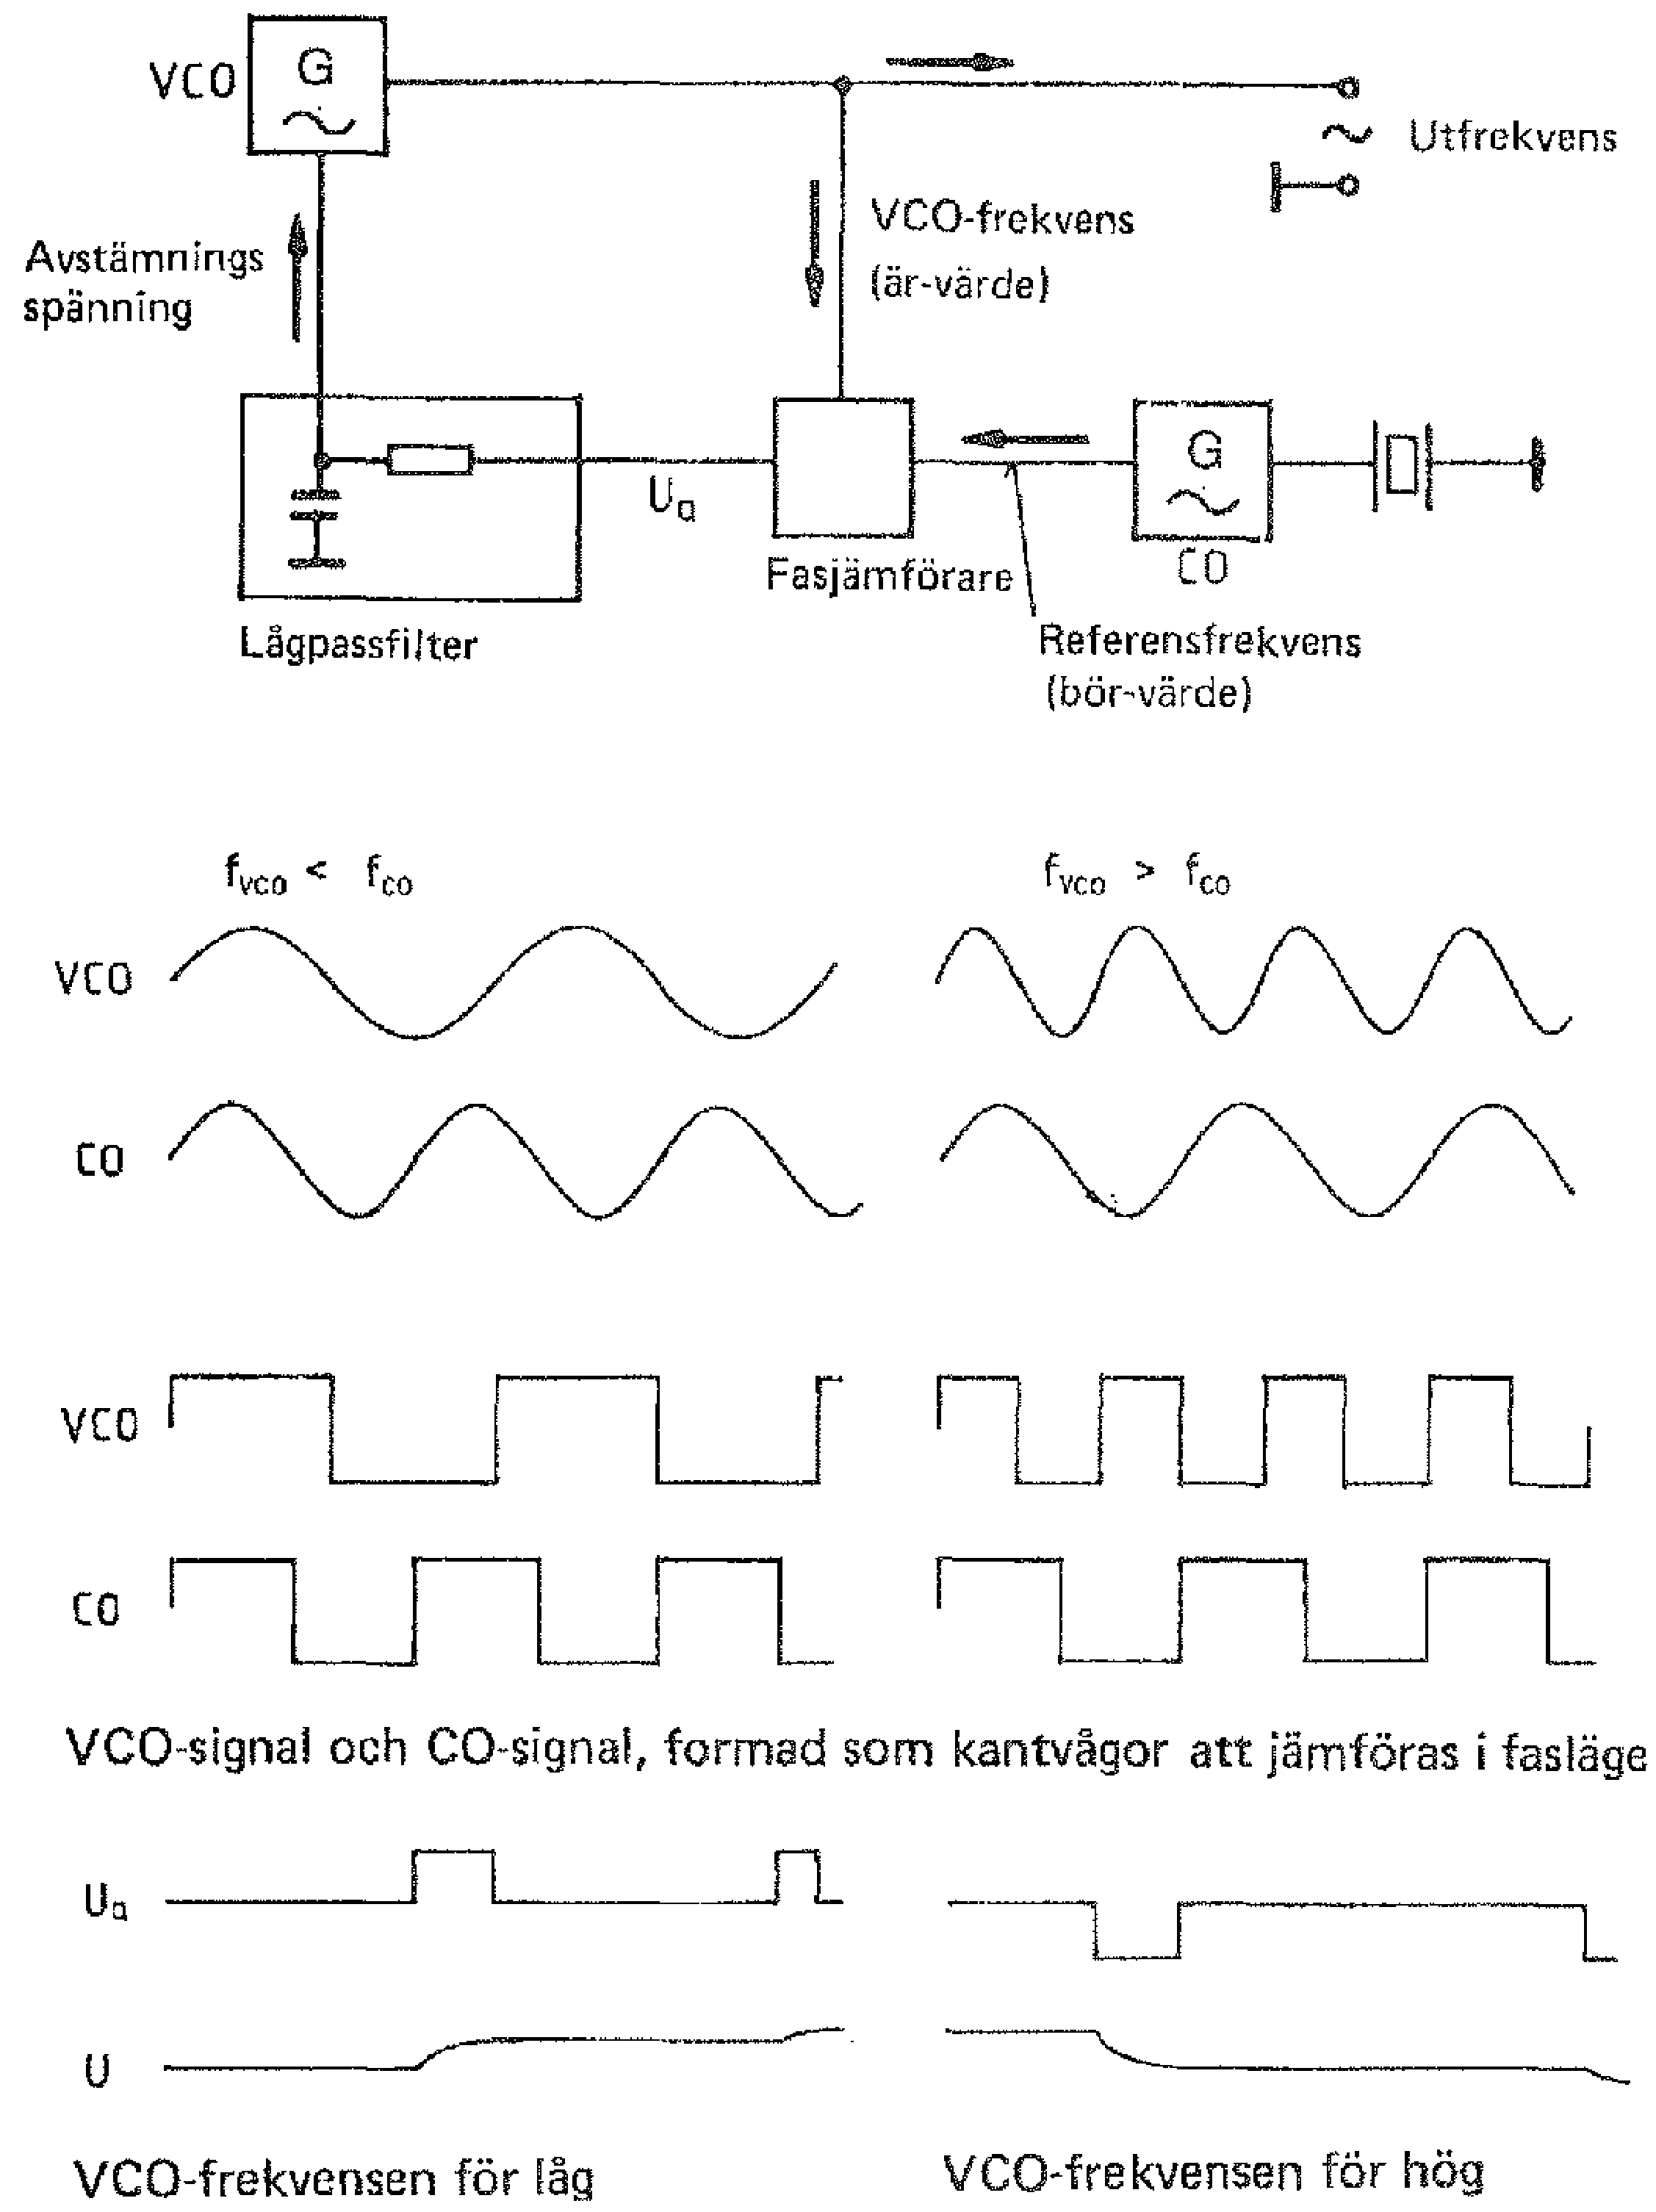
\includegraphics[width=\textwidth]{images/cropped_pdfs/bild_2_3-80b.pdf}
  \caption{Oscillator med PLL-styrning}
  \label{fig:BildII3-80b}
\end{figure}

Bild \ref{fig:BildII3-80b} illustrerar en oscillator med PLL-styrning.
Fasjämföraren levererar en cykliskt justerad styrspänning till
kapacitansdioden i VCO.
Eftersom denna spänning ändras språngvis, så avrundas förloppet så att
frekvensändringarna blir mjuka.
Avrundningen sker med ett RC-filter där kondensatorn antar ett medelvärde av den
pulserande utgångsspänningen från jämföraren.
Om VCO-frekvensen är för låg, så levererar jämföraren en positiv spänning.
Styrspänningen på kapacitansdioden stiger då med en hastighet som bestäms av
filtrets tidskonstant.

Kapacitansen i kapacitansdioden minskar med ökande spänning, eftersom
spärrskiktet blir tjockare och frekvensen på VCO stiger.

När signalen från VCO åter är lik referenssignalen från XO, till
fasläge och frekvens, så ökar utgångsresistansen i fasjämföraren.
Lågpassfiltrets kondensator behåller då sin laddning
och styrspänningen till VCO ändras inte t.v.
Skulle frekvensen på VCO vara för hög så blir jämförarens utgång lågohmig och
filtrets kondensator urladdas med den hastighet som bestäms av tidskonstanten.
Den sjunkande styrspänningen medför att kapacitansdiodens spärrskikt blir
tunnare, kapacitansen tilltar och VCO-frekvensen sjunker tills en ny fas- och
frekvenslikhet uppnåtts.

\subsubsection{PLL-oscillator i kombination med frekvensblandning}

\begin{figure}
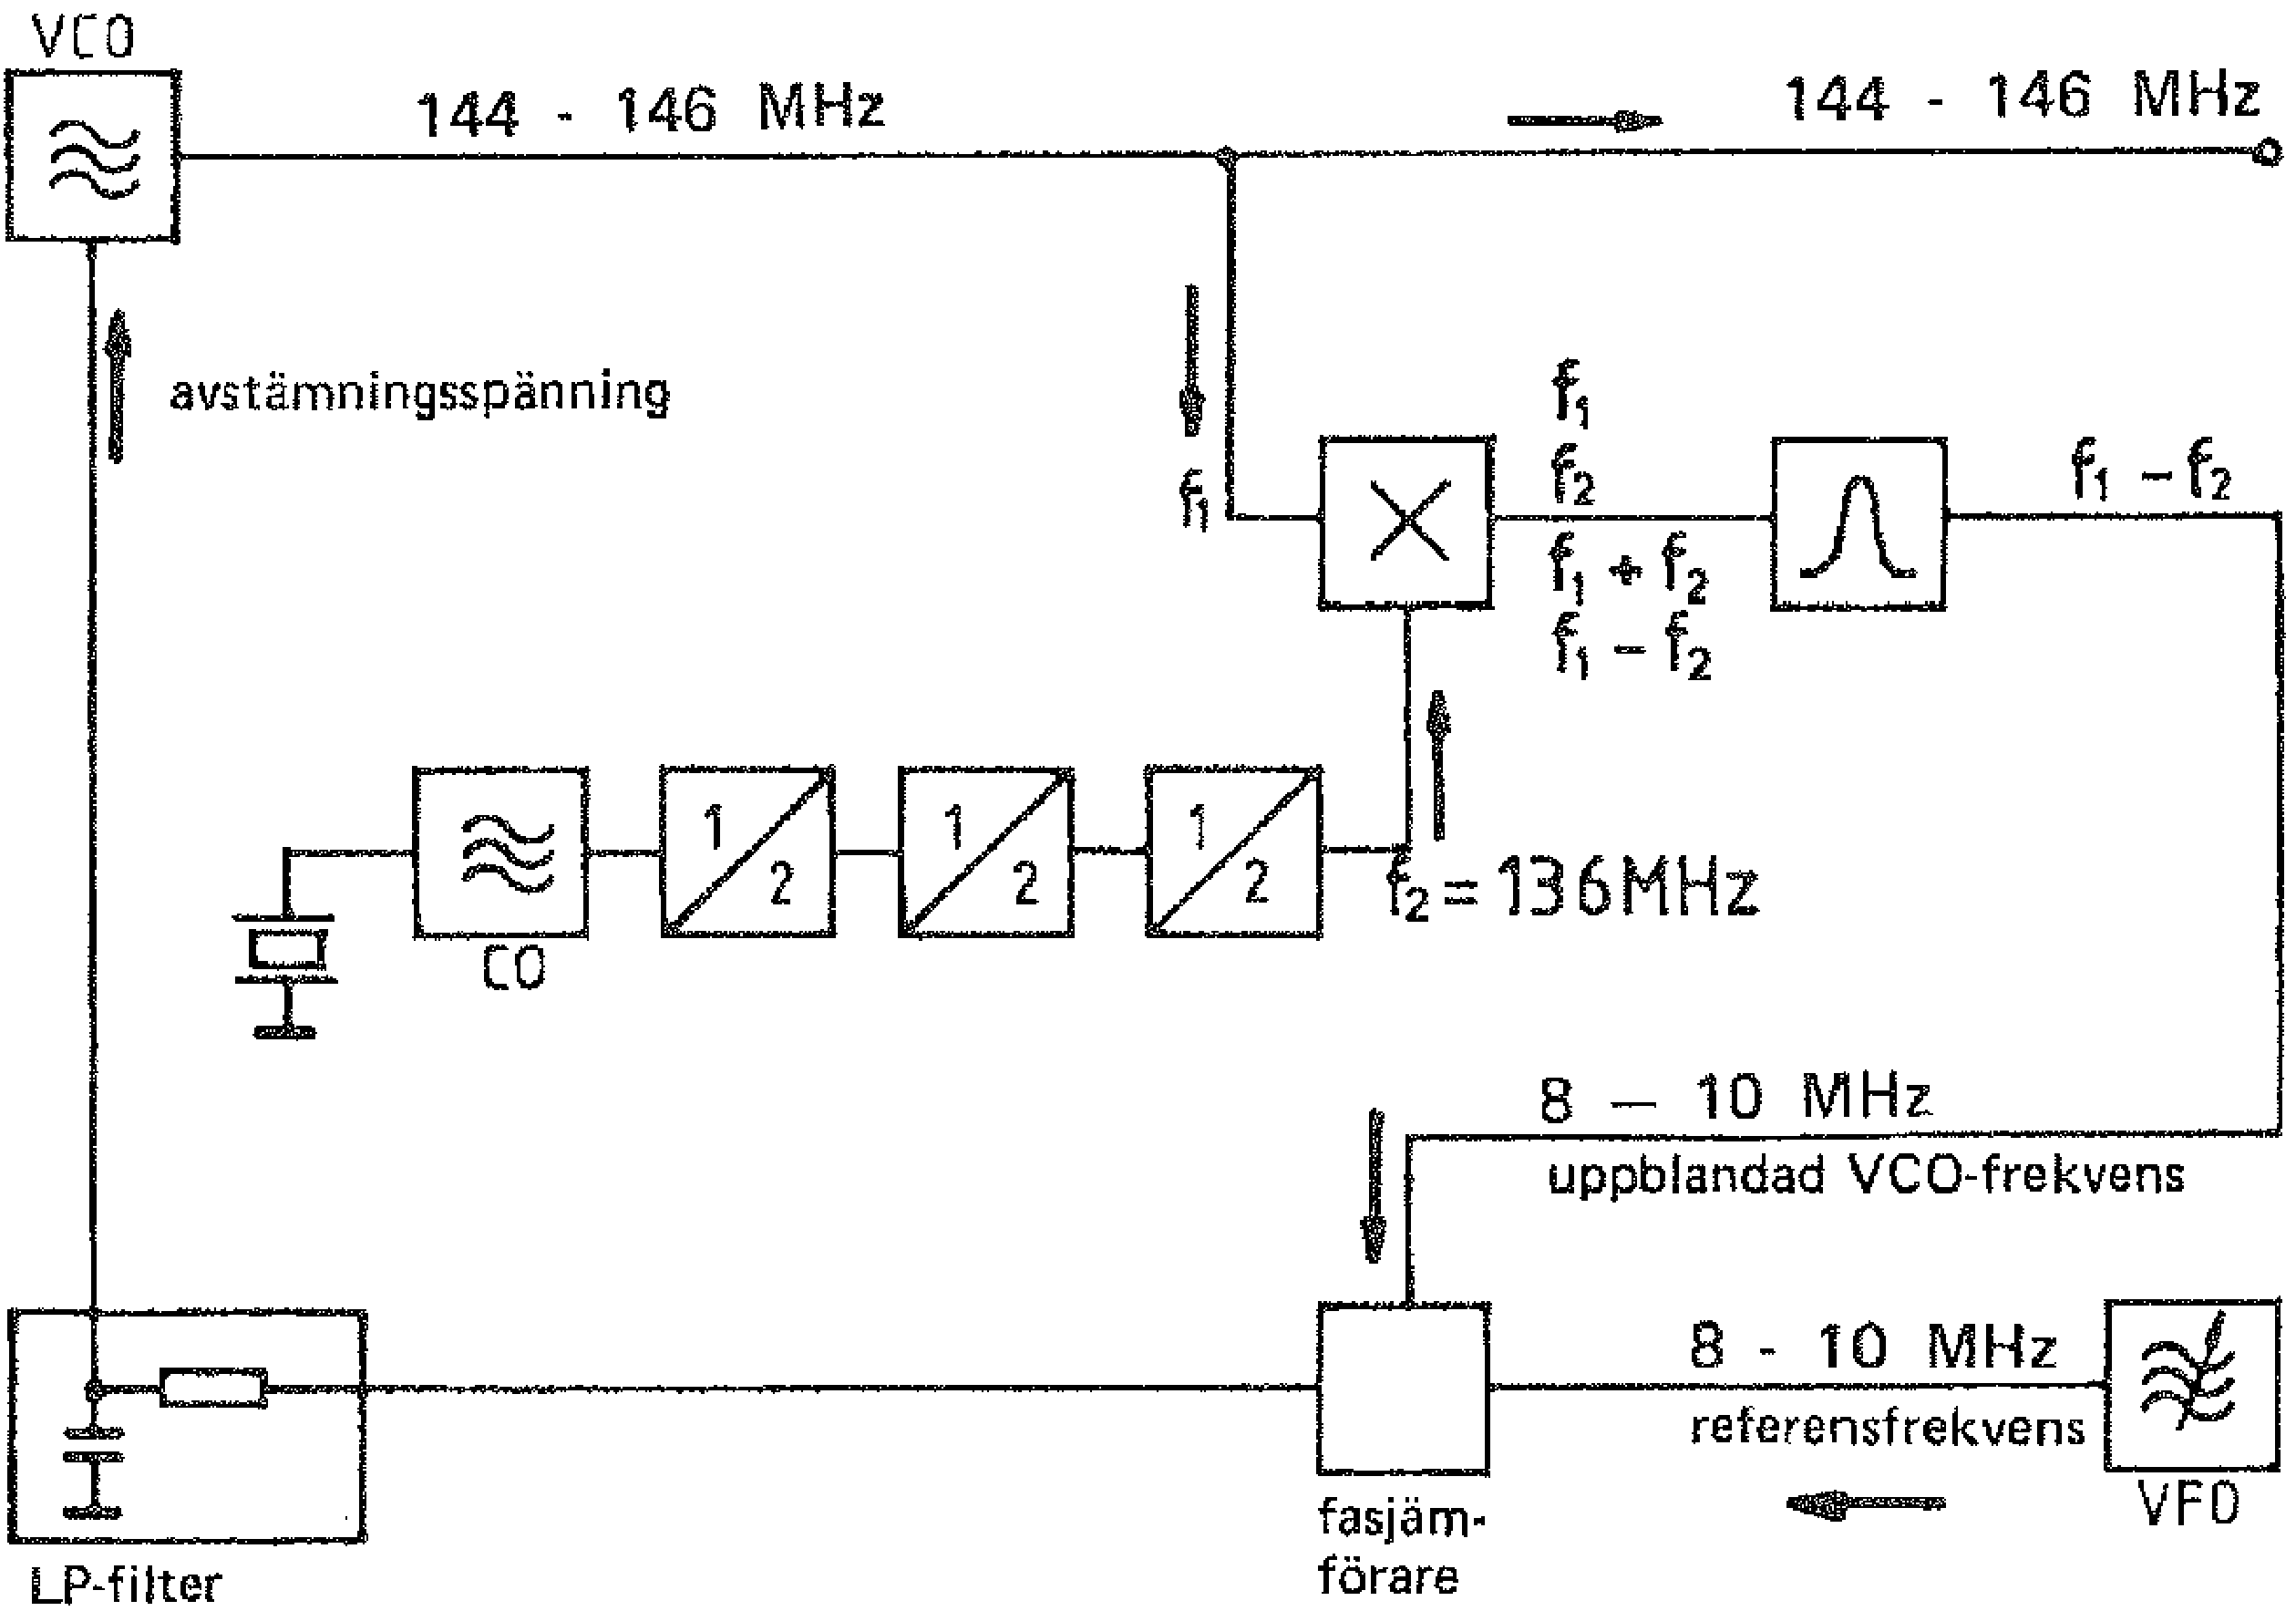
\includegraphics[width=\textwidth]{images/cropped_pdfs/bild_2_3-81.pdf}
\caption{PLL-oscillator kombinerad med frekvensblandning}
\label{fig:BildII3-81}
\end{figure}

Bild \ref{fig:BildII3-81} visar en PLL-oscillator kombinerad med
frekvensblandning.
Signalen \(f_1\) från en VCO alstrar en sändningsfrekvens i bandet
144--146~MHz.
Denna blandas med signalen \(f_2\) (136~MHz), som är en multiplicerad
XO-frekvens.
Blandningsprodukten \(f_1 - f_2\) filtreras fram, det vill säga en signal i
området 8--10~MHz som påförs en fasjämförare.
Utsignalen från en VFO, som är variabel inom samma frekvensområde 8--10~MHz,
påförs också fasjämföraren.

Utsignalen från jämföraren är en likspänning, som beror av frekvensskillnaden
mellan blandningsprodukt och VFO-signal.
Jämförarens utsignal ändras uppåt eller nedåt, beroende på frekvensfelets
riktning.

VCO-frekvensen bestäms av en likspänningsnivå, som styrs av jämförarens
utsignal.
Vid varje frekvensändring i VCO, kommer systemet att sträva mot
frekvensskillnaden noll i fasjämföraren vilket gör att sändningsfrekvensen
hålls vid rätt värde.

\textbf{Fördelar med en PLL-oscillator:}
Den har samma frekvensstabilitet som en VFO eftersom denna även här arbetar på
en låg frekvens.
Till skillnad mot en super-VFO finns inga sidofrekvenser i PLL-oscillatorn,
eftersom VCO alstrar nyttofrekvensen direkt.

\textbf{Nackdelar med en PLL-oscillator:}
Den har högre brusnivå än en super-VFO.
Frekvensstabiliteten är sämre än den för en PLL-oscillator med XO och
programmerbar frekvensdelare.

\subsubsection{PLL med programmerbar frekvensdelare}
\textbf{HAREC a.\ref{HAREC.a.3.7.2}\label{myHAREC.a.3.7.2}}
\index{PLL!programmerbar}

\begin{figure}
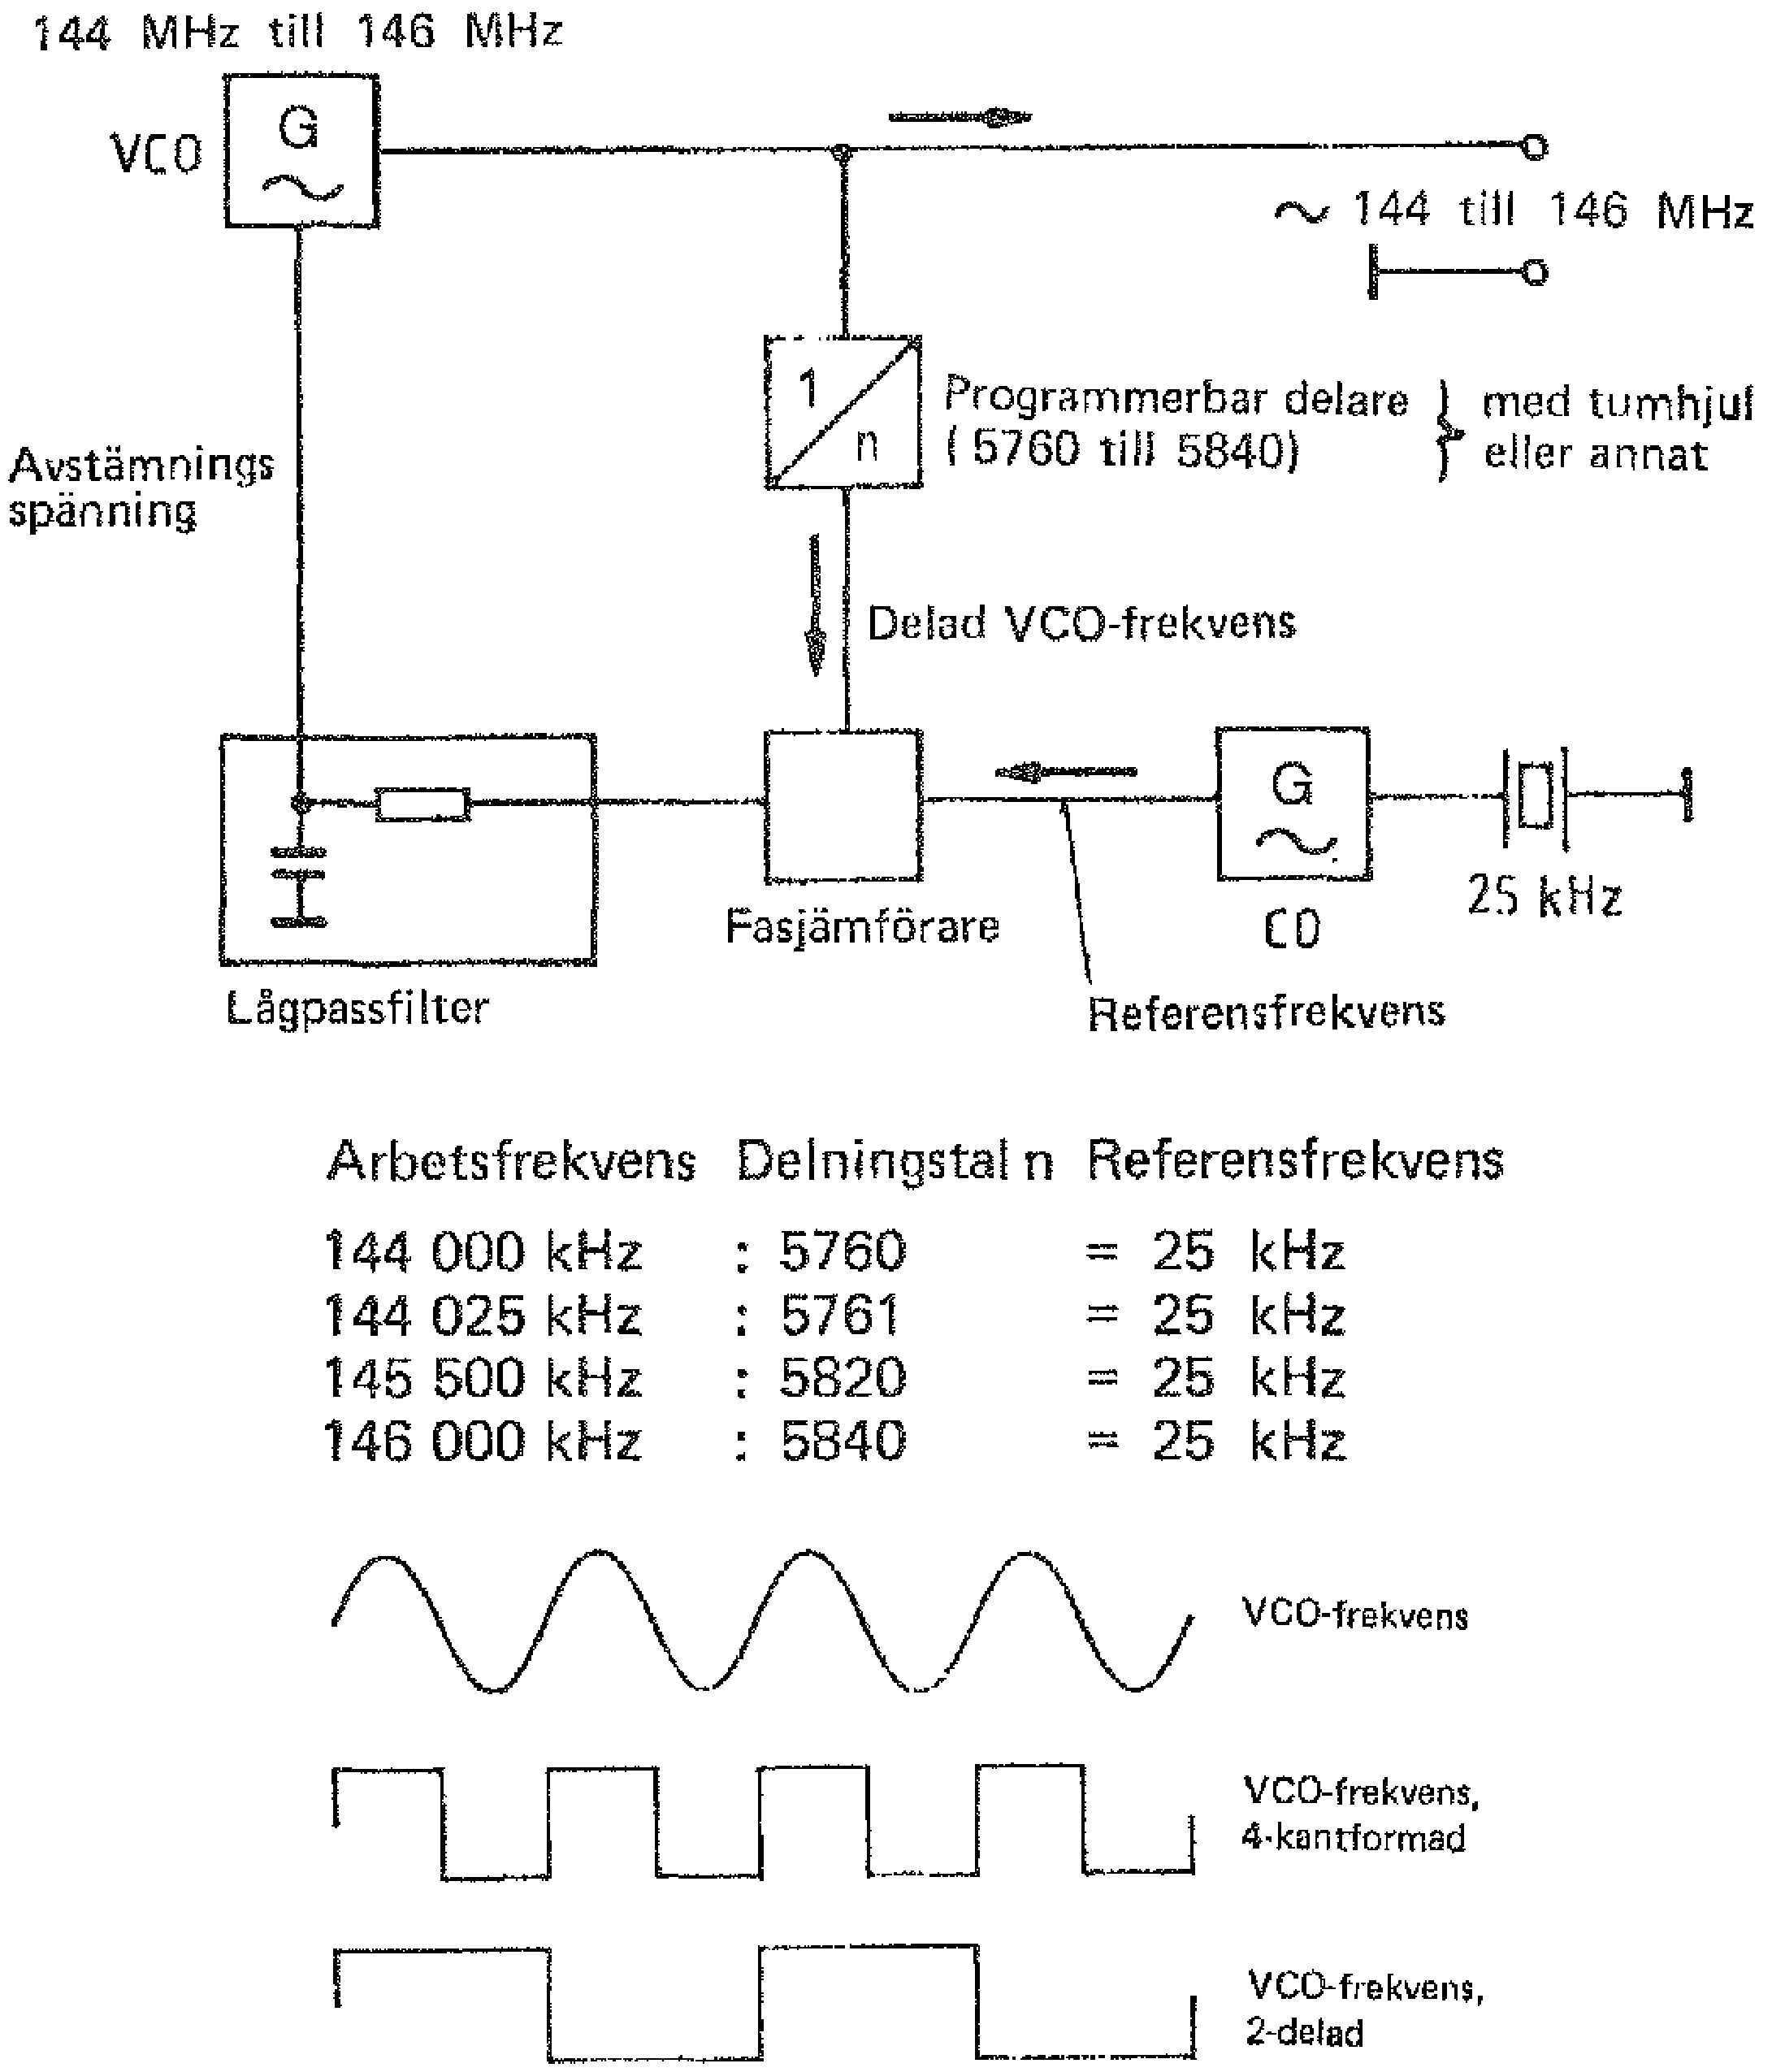
\includegraphics[width=\textwidth]{images/cropped_pdfs/bild_2_3-82.pdf}
\caption{PLL med frekvensdelare}
\label{fig:BildII3-82}
\end{figure}

Bild \ref{fig:BildII3-82} visar en PLL med frekvensdelare.
Med PLL blir frekvensen på utsignalen från en VCO låst till referensfrekvensen
från en XO.
I princip fås en VCO med samma frekvensstabilitet som en XO, men också lika
svår att ändra frekvensen på.
Med en frekvensdelare i fasregleringsslingan (PLL) kan emellertid utfrekvensen
ändras, medan XO fortfarande avger samma referensfrekvens.
En frekvensdelare är en digital krets, som räknar svängningar eller pulser upp
till ett valt tal för att återställas till i och börja om igen.
Vid varje återställning avges en utpuls.
Vid en delning med två avges en utpuls för varannan inpuls.
Vid delning med i 5 avges en utpuls för var i 5:e inpuls och så vidare.

Genom att välja delningstal i PLL kan arbetsfrekvensen i VCO ställas
in stegvis, där varje steg är så stort som en referensfrekvens.
Signalfrekvensen från vco delas med det valda delningstalet och resultatet
jämförs med referensfrekvensen från XO.
Varje avvikelse från likhet med referensfrekvensen kommer att
medföra justering av VCO-frekvensen.

Om man till exempel vill täcka 2-metersbandet i steg om 25~kHz, så väljer
man den referensfrekvensen samt att delaren kan fås att dela sändarens
utfrekvens med vilket som helst av talen 5760, 5761, 5762 osv. upp till 5840.
Om till exempel delningstalet 5820 valts, så kommer jämförarens styrspänning att styra
VCO-frekvensen till 145500~kHz.
Delarens utfrekvens blir då \(145500/5820 = 25\) kHz, vilket motsvarar
referensfrekvensen.
I detta exempel styrs alltså sändarens utfrekvens så att den alltid blir i steg
om 25~kHz.

\subsubsection{För- och nackdelar med PLL-oscillatorn}

PLL-oscillatorn har nästan samma frekvensstabilitet som en
kristalloscillator och frekvensen är inställbar i steg.
Till skillnad mot en VFO med mekaniskt inställbar frekvens, så är den PLL-styrda
VGO-oscillatorns frekvens elektroniskt inställbar.
Detta underlättar utformning och placering av reglage etc. för
frekvensinställning, frekvensminne och automatisk frekvensavsökning.

Först när den PLL-styrda oscillatorn kom till användning i handapparater och
mobila apparater blev det möjligt med frekvenstäckning över ett helt band med
bibehållet krav på små dimensioner.
Som jämförelse, skulle en inbyggnad av säg 80 till 800 stycken kanalkristaller
i en traditionell kristallstyrd apparat vara en mycket platskrävande, dyrbar
och opraktisk lösning.

Men PLL-oscillatorn brusar förhållandevis starkt jämfört med en VCO och
speciellt jämfört med en XO.
VCO-svängningskretsen har nämligen ett relativt lågt godhetstal eftersom en
kapacitansdiod belastar kretsen mer än en mekaniskt variabel kondensator.

Med det lägre godhetstalet blir svängningskretsen ett mindre bra
filter för dämpning av oscillatorbruset.
Kapacitansdioden tillför dessutom ett elektronbrus.
Därtill kommer det så kallade fasbruset från frekvensdelaren och PLL.

Med svängningskretsens låga godhetstal är frekvensstabiliteten i en VCO inte så
bra som den i en kristalloscillator, utan faktiskt sämre än den i en VFO.
Trots det är långtidsstabiliteten god i en VCO, när den ingår i en PLL,
eftersom att frekvensen hålls ständigt efterjusterad.
PLL kan däremot inte åstad- komma en lika bra korttidsstabilitet.
Ett fas- jämförelseförlopp omfattar ju redan tiden för en period av
referensfrekvensen.
Och det kommer att förflyta en multipel av denna kortaste tid innan
styrspänningen kan återställa VCO-frekvensen igen.
Detta beror på att kondensatorn i regleringsslingans lågpassfilter först måste
laddas upp under ett antal perioder innan reglering sker.

Dessa kortvariga frekvensavvikelser är en typ av frekvensmodulation
som leder till fasbrus från PLL-oscillatorn och som kan störa.
Det är dock endast i extrema fall som fasbruset verkar störande eftersom det
i moderna apparater reduceras till en acceptabel nivå genom noggrann
skärmning och filtrering.

\subsection{Faktorer som påverkar frekvensstabilitet}
\index{frekvensstabilitet}
\index{oscillator!stabilitet}

Sändarens frekvens ska hållas så stabil som möjligt.
En ostabil sändare är inte godtagbar och skapar svårigheter inte bara för de
radiostationer som deltar i förbindelsen utan även för radiotrafiken
på närliggande frekvenser.

En frekvensstabil oscillator ska ha följande egenskaper:

\subsubsection{Stabil mekanisk uppbyggnad}

Skakningar från underlaget till exempel vid mobilt bruk, vibrationer från en
transformatorkärna etc. kan försämra oscillatorns frekvensstabilitet.

Frekvensbestämmande komponenter såsom fasta och variabla kondensatorer, spolar
etc. ska vara stabilt monterade, trimkärnorna i spolarna fixerade osv.

Förbindningarna får inte tillåtas att böja sig eller vibrera.
Apparatstommen måste vara tillräckligt styv för att inte ändra formen och
därigenom medföra frekvensändringar vid hantering osv.

\subsubsection{God elektrisk uppbyggnad och högt Q-värde i svängningskretsarna}

Alla elektriska förbindningar måste vara så korta som möjligt och löd-
och kopplingsställen fullgoda.
Induktorer och kondensatorer i svängningskretsarna måste vara förlustfattiga
och högvärdiga i övrigt så att signalen blir så ren som möjligt från oönskade
sidofrekvenser.

Återkopplingen i oscillatorn ska vara så fast (kraftig) att självsvängningen
är stabil.
Men för att få en renast möjlig signal får kopplingen inte vara så fast,
att svängningskretsarna blir alltför belastade och deras godhetstal för lågt.

\subsubsection{Avskärmande kapslingar}

Svängningskretsar ska skärmas från yttre kapacitanstillskott
(t.ex. från en hand).
Det görs med skiljeväggar och komponentkapslingar av metall.
Skärmningarna förhindrar också oönskad koppling mellan oscillatorn och
efterföljande förstärkare genom elektriska och magnetiska fält.

\subsubsection{Stabila drivspänningar}

Ostabila drivspänningar medför frekvensändringar.
I en oscillator med transistorförstärkare beror ostabiliteten på förändringar
mellan skikten i en transistors diodsträcka.
Skikten fungerar nämligen som ''kondensatorplattor'' och spärrskiktet där
emellan som dielektrikum.
Tjockleken av spärrskiktet och därmed ''plattavståndet'' står i förhållande
till den spänning som läggs över transistorn.
Den spänningsberoende kapacitansen i transistorn är ansluten till
svängningskretsen via kopplingskondensatorn.

Eftersom kapacitansen i transistorn är en del av svängningskretsen, så påverkar
den resonansfrekvensen.
Denna egenskap kan vara till besvär, men kan även användas för att på ett
enkelt sätt ändra oscillatorns arbetsfrekvens.
Se Kapacitansdiod och PLL-oscillatorn.

\subsubsection{Buffertsteg}

En oscillator i en radiosändare kan bestå av ett enda förstärkarsteg,
som alstrar högfrekventa elektriska svängningar.
Vanligen tas endast små effekter ut från en så enkel sändare, normalt mindre än
en watt.
Utan särskilda åtgärder, som till exempel att använda en styrkristall, är nämligen
frekvensen inte särskilt stabil och olämplig för kommunikationsändamål.

Särskilt varierande belastning över oscillatorns utgång medför frekvensändring.
Oscillatorn bör därför ges en så låg och stabil belastning som möjligt.
Ett buffertsteg kopplas därför in efter oscillatorn.
Det bör ha hög ingångsimpedans för att belasta oscillatorn så lite som möjligt.
Det ska också kunna lämna tillräcklig driveffekt till efterföljande förstärkare
och bör därför ha låg utgångs impedans.
Det måste dessutom arbeta linjärt (se klass A-drift, bild \ref{fig:BildII3-44})
för att inte alstra övertoner och därmed förvränga oscillatorsignalen.
Bild \ref{fig:BildII3-42} visar ett buffertsteg i kollektorkoppling, vilken har
dessa egenskaper.

\subsubsection{Temperaturkompensation och termostater}

Det alstras alltid förlustvärme i elektriska apparater och även i en
oscillator.
Vid uppvärmningen utvidgas spolar och kondensatorer i svängningskretsarna,
vilket leder till frekvensändringar.
Även spärrskiktskapacitansen i transistorerna är temperaturberoende.
Det totala temperaturberoendet kan kompenseras genom ett antal åtgärder.

Oscillatorn bör monteras så långt bort som möjligt från övriga
värmealstrande komponenter.
Den avskärmande kapslingen omkring oscillatorn ska vara så tjockväggig och
värmeisolerande som möjligt.
Inbyggnad i en termostatreglerad kapsling är ett ännu bättre alternativ.

Komponenterna bör ha uppnått drifttemperatur för användningen.
Oscillatorn bör därför värmas upp under åtminstone 15~minuter.

\subsection{Frekvensstabilitet och oscillatorbrus}
\textbf{HAREC a.\ref{HAREC.a.3.6.6}\label{myHAREC.a.3.6.6}}

Frekvensstabiliteten i kristalloscillatorer är ca 100 gånger bättre än
den är i LC-oscillatorer.
Likaså är utgångssignalen från kristalloscillatorer renare från så kallat
fasbrus (jitter).
Varje oscillator avger nämligen även oönskade signaler med frekvenser som
ligger omkring utgångssignalens nominella frekvens.

Oscillatorn är ju en förstärkare, vars utgångsspänning delvis
återkopplas till ingången i medtas.
Detta innebär att utgångssignalen förstärks lavinartat till ett maximum,
omväxlande med att den dämpas lavinartat till ett minimum.
Utan yttre påverkan befinner sig alltså förstärkaren i ett
självsvängningstillstånd mellan två yttervärden.
I återkopplingsvägen placeras ett filter som frekvensbestämmande
element, till exempel en LC-krets eller en kvartskristall.

Återkopplingen blir starkast på filtrets resonansfrekvens, vilket
medför att oscillatorn svänger bäst där.
Eftersom filtret oundvikligen har en viss bandbredd, så kommer även ett
spektrum av andra frekvenser tätt omkring resonansfrekvensen att släppas
igenom.
De oönskade frekvenserna omkring den nominella kallas för brus.

I moderna konstruktioner används oftast PLL-oscillatorer.
På grund av sin funktion pendlar deras frekvens alltid något.
Hur mycket beror bland annat på loop-filtret.
Alltså är frekvensen egentligen ett mycket litet band av flera frekvenser varav
en framträder mest.

\textbf{Försök:}

Volymkontrollen i en lågfrekvensförstärkare utan insignal vrids till maximum.
Det kommer att höras ett brus i högtalaren, som huvudsakligen kommer från
ingångsstegets transistorer.
När en mikrofon ansluts måste volymkontrollen vridas ner och då hörs bruset
mindre.
Men bruset finns ändå där på en lägre nivå och överlagras på insignalen från
mikrofonen.

Även i en högfrekvensoscillator överlagras bruset på insignalen.
Men ju högre godhetstalet är i svängningskretsen, till exempel en kristall, desto
smalare är filtrets bandbredd, desto kraftigare blir brusundertryckningen och
desto mer framhävs den önskade signalen.
P.g.a. det större godhetstalet i svängningskretsen, och därmed den mindre
bandbredden, så brusar alltså en kristalloscillator mindre än en LC-oscillator.

En nackdel med kristalloscillatorn är att dess frekvens inte kan
ändras inom ett större område.
Önskas flera valbara frekvenser från en kristalloscillator måste flera
kristaller användas tillsammans med något slags omkopplingsanordning
(kanalväljare).

Komponentmängden i en kristalloscillator är mindre än i en VFO, men i
apparater för flera frekvenser uppvägs denna fördel av merkostnaden
för flera kristaller och kanalväljaren.

Kristalloscillatorn har många användningsområden, där en
frekvensstabil och brusfattig signal önskas och där platsbrist,
skakningar med mera utesluter användning av en LC-VFO.
